\documentclass[a4paper,12pt,russian]{article} %draft
\usepackage[T2A]{fontenc}% Поддержка русских букв


% XeTeX packages
\usepackage[cm-default]{fontspec} % or install lmodern and remove cm-default opt
\usepackage{xunicode} % some extra unicode support
\usepackage{xltxtra} % \XeLaTeX macro


\tolerance=1000
\emergencystretch=0.74cm
\usepackage{indentfirst} %делать отступ в начале параграфа

\usepackage[pdfborder = {0 0 0}]{hyperref} %гиперссылки в документе.

\usepackage[utf8]{inputenc}	% кодировка текста
\usepackage[russian]{babel}	% руссификация по Бабелю
\usepackage{graphics}

\usepackage[clean,pdf]{svg}

\usepackage{amsmath, amsfonts} % для расширенных настроек ссылок на формулы
\usepackage{extsizes}	% использование шрифтов большего кегля 

\usepackage{fancyvrb} % Добавляет продвинутые Verbatim и Verb

\usepackage{epsfig} % удобно вставлять рисунки в строку текста
\usepackage[usenames,dvipsnames]{pstricks}
\usepackage{pst-grad} % For gradients
\usepackage{pst-plot} % For axes

\usepackage{graphicx,xcolor}

%\usepackage[MakeStamp]{eskdi}
%\usepackage[MakeStamp, SubSectInToc]{eskdi}
%\usepackage[MakeStamp, SubSubSectInToc]{eskdi}
%\usepackage[MakeStamp, ParagraphInToc]{eskdi}
%\usepackage[twoside, MakeStamp, ParagraphInToc]{eskdi}
%\usepackage{eskdi}
%\usepackage[SubSectInToc]{eskdi}
%\usepackage[SubSubSectInToc]{eskdi}
%\usepackage[ParagraphInToc]{eskdi}
%\usepackage[ParagraphInToc, NumIntoSections]{eskdi}
%\usepackage[twoside, ParagraphInToc]{eskdi}
%\usepackage[twoside, MakeEmptyStamp, ParagraphInToc]{eskdi}
\usepackage[twoside, MakeEmptyStamp]{eskdi}
%\usepackage[MakeEmptyStamp, ParagraphInToc]{eskdi}



\usepackage{array}
\usepackage{tabularx}
\usepackage{supertabular}
\usepackage{longtable} % для создания таблиц, переносящихся на другую страницу
%\usepackage{listingsutf8}%
\usepackage{listings} % для включения листинга кода в приложения. Русский язык глючит.


\lstloadlanguages{bash,[LaTeX]TeX,MetaPost,Clean,Matlab}


\usepackage{textcomp}	% Ввод различных знаков
\usepackage{keystroke} % для отображения символов клавиш
\usepackage{bytefield} %для создания таблиц с битовыми полями
\usepackage{filecontents} %для включения в документ содержимого файлов

\usepackage{tikz} % Пакет для рмсования диаграмм
\usepackage{tikz-timing}[2009/12/09]
\usetikzlibrary{positioning,arrows,automata,plotmarks} %В данном случае нам потребуются positioning и arrows, которые нужны для расположения элементов друг относительно друга и рисования стрелок между ними соответственно.
\usetikzlibrary{shapes,snakes}
\usepackage{schemabloc}

\usepackage{makecell} % Для многострочных ячеек таблицы
\usepackage{colortbl} % Для раскрашивания ячеек в таблицах


%{Arial} {Courier New} 
%{OpenGost Type A TT} {OpenGost Type B TT} % Свободный шрифт. Нет наклонного начертания и дирного начертания
%{GOST type A} % Морально устарел, не свободный, не хватает символа тирэ. Не рекомендуется
%{GOST type B} % Морально устарел, не свободный, не хватает символа тирэ. Не рекомендуется
\gostSetRomanfont{Times New Roman}%
\gostSetSansfont{Times New Roman}%
\gostSetMonofont{Times New Roman}%
\gostSetMainfont{Times New Roman}%
\gostSetStampfont{Arial}%


%\verbatimfont{\fontspec[Scale=1.0]{Arial} \itshape}% % Для замены стиля начертания verbatim и verb
\verbatimfont{\fontspec[Scale=1.0]{Consolas}}% % Для замены стиля начертания verbatim и verb
\newfontfamily{\gostListingfont}[Scale=1.0]{Consolas} % Шрифт для листингов
%\renewcommand{\SetStampfontIt}{\itshape}%

%\input commands.tex %Файл включает такие команды как надчёркивание, запрещение переноса ТУ и др.
\setpage % Разметка текста на странице
\begin{document}

	\gosttitleobject{Лабораторная работа}
		
	\gosttitledocument{МОДЕЛИРОВАНИЕ ЛИНЕЙНЫХ ДИНАМИЧЕСКИХ СИСТЕМ}

	% Раскомментировать если необходима утверждающая надпись на титульном листе
	\renewcommand\titleBotRIGHT{
	\spboxmm{100}{70}{70}{30}{lc}{\parbox{70mm}{
			\normalsize{Преподаватель: Чепинский С.А. }\\ 
			\normalsize{Студенты: Французов Р.А.\\  Донцова М.А.}\\
			\normalsize{Группа: R3325}\\
			\normalsize{Вариант: 18}}}}

		\maketitle
		
		\section{Цель работы}
		Ознакомление с пакетом прикладных программ SIMULINK и основными приемами моделирования линейных динамических систем. \\
		
		\section{Ход работы}
Ниже представлены исходные данные варианта для системы вход-выход\\
\begin{center}
\begin{tabular}{|c|c|}
	\hline
	$a_0$ & 15 \\ \hline
	$a_1$ & 5 \\ \hline
	$a_2$ & 10 \\ \hline
	$b_0$ & 15 \\ \hline
	$b_1$ & 0.5 \\ \hline
	$b_2$ & 1 \\ \hline
	$y(0)$ & 1 \\ \hline
	$\dot{y}(0)$ & 0.5 \\ \hline
	$\ddot{y}(0)$ & 0.1\\ \hline
\end{tabular}
\end{center}
и вход-состояние-выход\\
\begin{center}
	\begin{tabular}{|c|c|}
		\hline
		$A$ & $\begin{pmatrix}0& -12\\1& -0.8\end{pmatrix}$ \\ \hline
		$B$ & $\begin{pmatrix}2\\0\end{pmatrix}$ \\ \hline
		$C^T$ & $\begin{pmatrix}3\\0.1\end{pmatrix}$ \\ \hline
		$x_1(0)$ & 0.33 \\ \hline
		$x_2(0)$ & -0.5 \\ \hline
	\end{tabular}
\end{center}

\subsection{Моделирование системы вход-выход}
По исходным данным варианта составлено и упрощено уравнение:\\
$y^{(3)}+10\ddot{y}+5\dot{y}+15y=\ddot{u}+0.5\dot{u}+15u\\
s^3y+10s^2y+5sy+15y=s^2u+0.5su+15u\\
s^3y=s^2(u-10y)+s(0.5-5y)+(15u-15y)\\
y=\dfrac{1}{s}(u-10y)+\dfrac{1}{s^2}(0.5-5y)+\dfrac{1}{s^3}(15u-15y)\\$

Основываясь на последнем уравнении составлена схема моделирования системы и проведены симуляции при входных воздействиях $u=1(t)$ и $u=2sin(t)$:\\ 
\begin{figure}[H]
	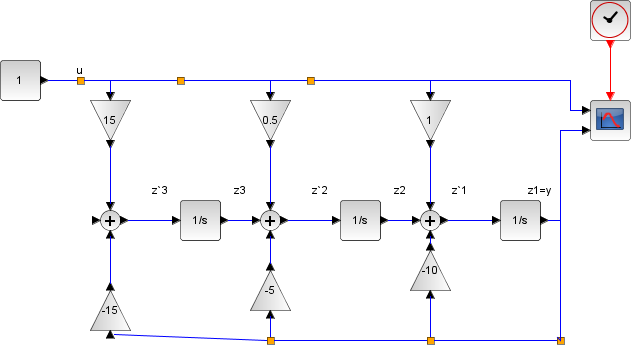
\includegraphics[width=1\textwidth]{вход-выход-схема}
	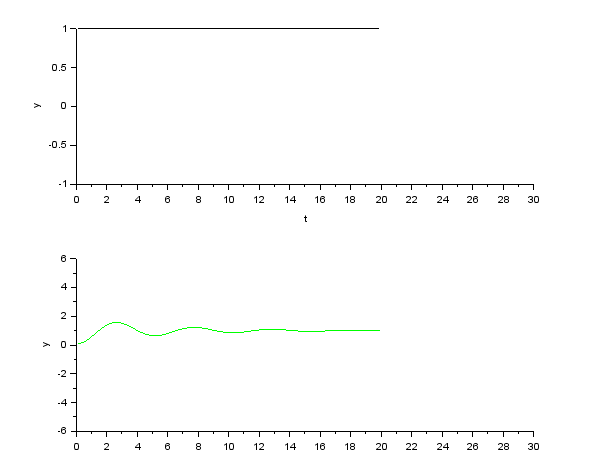
\includegraphics[width=1\textwidth]{вход-выход-1}
	\caption{Схема и результаты моделирования при единичном воздействии}
\end{figure}
\begin{figure}[H]
	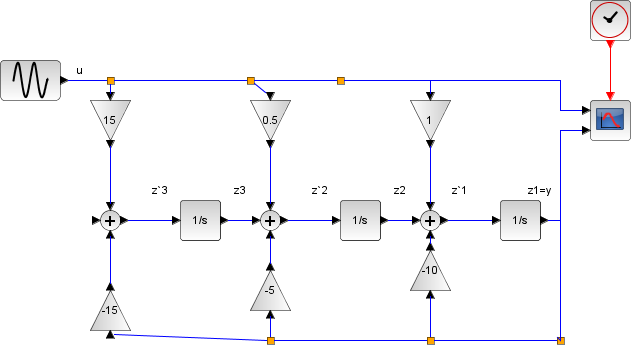
\includegraphics[width=1\textwidth]{вход-выход-схема-sin}
	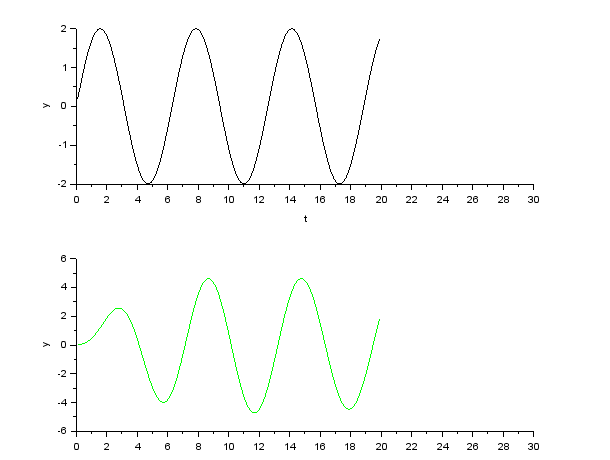
\includegraphics[width=1\textwidth]{вход-выход-sin}
	\caption{Схема и результаты моделирования при   $u=2sin(t)$}
\end{figure}
Для моделирования свободного движения системы были найдены начальные условия для интеграторов:\\
$z_1=y \rightarrow z_1(0)=y(0)=1\\
\dot{z_1}=z_2+u-10y \rightarrow z_2=\dot{y}-u+10y \rightarrow z_2(0)=10.5\\
\dot{z_2}=z_3+0.5u-5y \rightarrow z_3=\dot{z_2}-0.5u+5y \rightarrow z_3(0)=15.5\\$
\begin{figure}[H]
	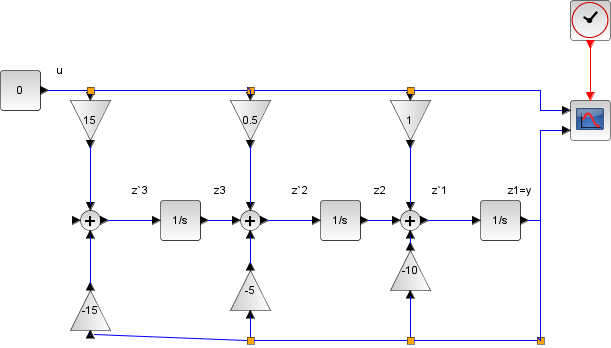
\includegraphics[width=1\textwidth]{вход-выход-схема-св}
	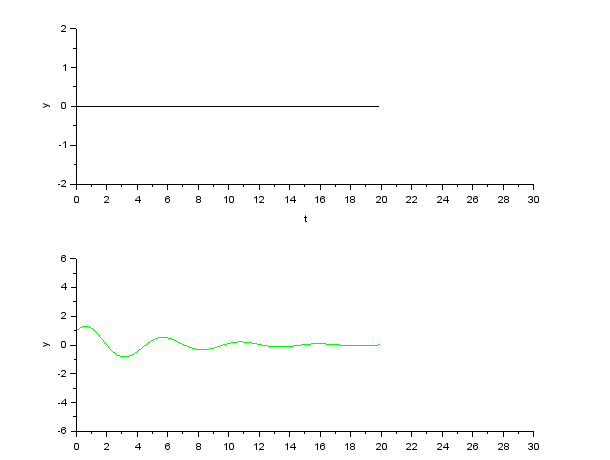
\includegraphics[width=1\textwidth]{вход-выход-св}
	\caption{Схема и результаты моделирования свободного движения системы}
\end{figure}

\subsection{Моделирование системы вход-состояние-выход}
По исходным данным варианта составлена система уравнений:\\
$\begin{cases}\dot{x_1}=-12x_2+2u\\\dot{x_2}=x_1-0.8x_2\\y=3x_1+0.1x_2\\\end{cases}$\\
Основываясь на системе уравнений составлена схема моделирования системы и проведены симуляции при входных воздействиях $u=1(t)$ и $u=2sin(t)$, а также свободного движения системы:\\ 
\begin{figure}[H]
	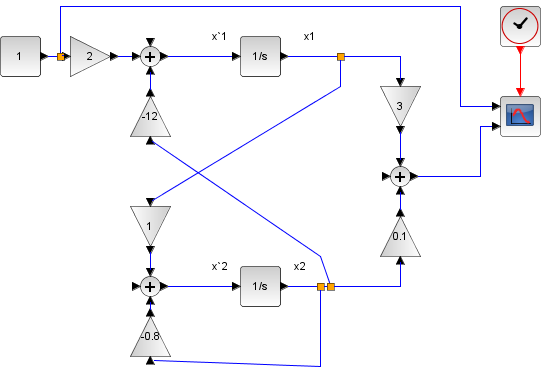
\includegraphics[width=1\textwidth]{всв-схема}
	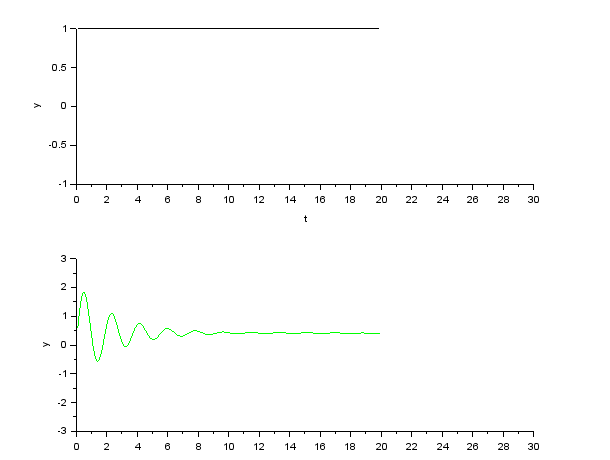
\includegraphics[width=1\textwidth]{всв-1}
	\caption{Схема и результаты моделирования при единичном воздействии}
\end{figure}
\begin{figure}[H]
	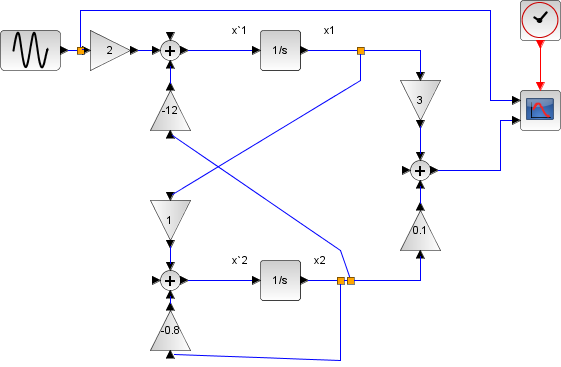
\includegraphics[width=1\textwidth]{всв-схема-sin}
	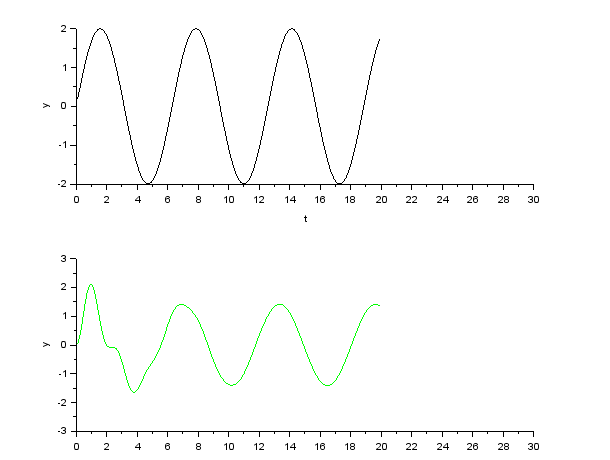
\includegraphics[width=1\textwidth]{всв-sin}
	\caption{Схема и результаты моделирования при   $u=2sin(t)$}
\end{figure}
\begin{figure}[H]
	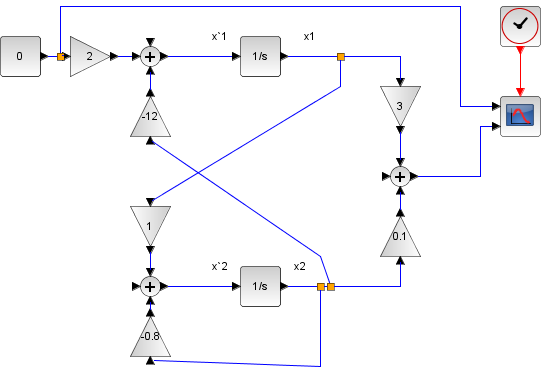
\includegraphics[width=1\textwidth]{всв-схема-св}
	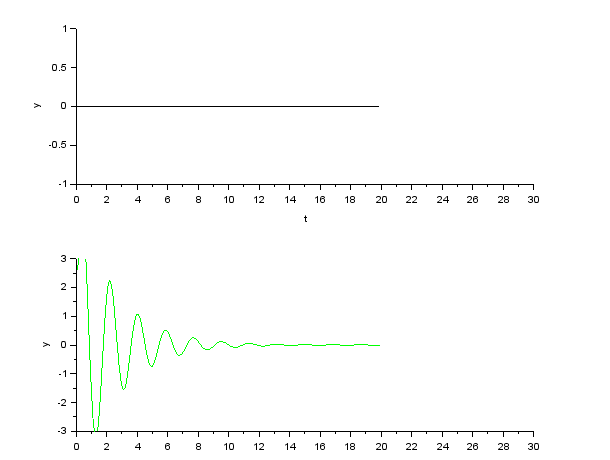
\includegraphics[width=1\textwidth]{всв-св}
	\caption{Схема и результаты моделирования свободного движения системы}
\end{figure}


\section{Вывод}
В данной лабораторной работе были построены схемы моделирования систем вида вход-выход и вход-состояние-выход, проведены симуляции переходных процессов при различных входных воздействиях и свободного движения.
\end{document}